\scanpage{27}
\begingroup\makeatletter\tagsleft@true\makeatother
\margin{
\begin{tikzpicture}
\node[inner sep=1pt,align=left,text width=.93\marginparwidth] (titre) {filtered structure on de Rham and comparison with Betti, Hodge...};
\draw (titre.north west) -- (titre.south west) -- (titre.south east);
\end{tikzpicture}}

Let $k\unsure{\mathrel{\tikz[x=.58em,y=.58em,baseline=0pt,line cap=round]{\draw (.87,.44) .. controls (.60,.70) and (-.03,.34) .. (.04,.17) .. controls (.12,.04) and (.78,.09) .. (1.20,.02); \draw (1.23,.14) -- (1.14,.80) .. controls (1.15,.96) and (.92,.79) .. (.99,1.00) .. controls (1.01,1.08) and (1.05,1.12) .. (1.09,1.13);}}|\subset^{\iota}|\subset}\mathbb{C}$, let us consider a category of motives \inserted{over $k$,} of finite type \deleted{\unsure{say}}, say $\mathcal{M}$. There are two natural fibre functors,
\[
T_{\mathrm{DR}}:\mathcal{M}\relbar\operatorname{Mod}f(k)\tag*{(1)}
\]
\diagram{\begin{minipage}{\linewidth}
\[
\begin{tikzcd}[ampersand replacement=\&,column sep=1.2em]
T_{B\unsure{\mathrm{dg}|\mathrm{Hdg}|\mathrm{tg}}}:\mathcal{M}\arrow[r]\&
\deleted{\operatorname{Mod}f(\unsure{\mathbb Q|Q})}\ \mathrm{Str.}\ \mathrm{Hodge}\arrow[r]\&
\operatorname{Mod}f(\mathbb Q),
\end{tikzcd}\tag*{(2)}
\]
\end{minipage}}
the second depending on the embedding $k\subset\mathbb{C}$. The first has a filtration structure. Moreover, one has a canonical isomorphism
\[
\varphi:T_B\otimes_{\mathbb Q}\mathbb C\xrightarrow{\sim}T_{\mathrm{DR}}\otimes_k\mathbb C\tag*{(3)}
\]
\inserted{compatible with the filtrations of the 2 \unsure{sides|sides}}

Let $G$ be the group of automorphisms of $T_B$. Comparing $T_{\mathrm{DR}}$ and $T_B\otimes_{\mathbb Q}k$, one finds a right torsor
\[
P=\unsure{\underline{\operatorname{Isom}}|\underrightarrow{\operatorname{Isom}}}_{\otimes}(T_B\otimes_{\mathbb Q}k,T_{\mathrm{DR}})\tag*{(4)}
\]
under $G_k$, which allows one to recover the functor $T_{\mathrm{DR}}$ as
\[
T_{\mathrm{DR}}=\deleted{T_B\otimes}\ P\overset{G_k}{\times}(T_B\otimes_{\mathbb Q}k).\tag*{(5)}
\]
Moreover, \deleted{\unsure{one has an isomorphism}} the isomorphism (3) defines a canonical element
\[
\varphi\in P(\mathbb C)
\]
\margin{\begin{tikzpicture}
\node[inner sep=1pt,align=left,text width=.91\marginparwidth] (note) {Knowledge of $G,P,\varphi$ allows one essentially to recover $\mathcal M$ with (1) (2) and (3)};
\draw ([xshift=1pt]note.north west) -- ([xshift=-3pt]note.south west);
\end{tikzpicture}}% slanted

To recover the filtered structure on $T_{\mathrm{DR}}$, \deleted{and} hence the Hodge structure on $T_B$ i.e the bigrading on $T_B\otimes_{\mathbb Q}C$, it is appropriate to introduce
\[
T_{\mathrm{Hdg}}\unsure{\in|\mathord{:}}\mathcal M\longrightarrow\operatorname{Mod}\deleted{\unsure{\mathrm{Bi}|\mathrm B}}\mathrm{grad}\,f(k),\qquad T_{\mathrm{Hdg}}=\operatorname{gr}^{*}T_{\mathrm{DR}}.\tag*{(6)}
\]
\inserted{Let} \deleted{and the two \unsure{groups|groups} of} \deleted{Lie}
\[
\deleted{\unsure{H|K}}\ G'_k=P\overset{G_k}{\times}G_k=\operatorname{ad}(P)\simeq\underline{\operatorname{Aut}}_{\otimes}(T_{\mathrm{DR}})\tag*{(7)}
\]
\deleted{\unsure{Thus|Then}} and
\[
\begin{aligned}
H'\subset G'_k\qquad &\text{subgroup of the $\otimes$-automorphisms of $T_{\mathrm{DR}}$ preserving}\\
&\text{the filtration and which induce the}\\
&\text{identity on the associated graded.}
\end{aligned}\tag*{(8)}
\]
\endgroup
% archive sheet number: 26
